O ADC (\emph{Analog-To-Digital Converter}) é um periférico responsável por realizar a conversão de uma grandeza analógica de tensão para um valor correspondente digital. Para realizar esta conversão podemos implementar vários  tipos circuito, como o conversor flash, ou o conversor de aproximações sucessivas, ou ainda conversor integrador simples e de rampa dupla. Porém o  circuito de conversão mais usado em circuito integrados atualmente é o conversor de aproximações sucessivas, o qual também usado como AD no Tiva TM4C1294NCPDT. A figura \ref{fig:ConversorAD} apresenta o circuito em questão.


\begin{figure}[H]
	\centering
	\fbox{
	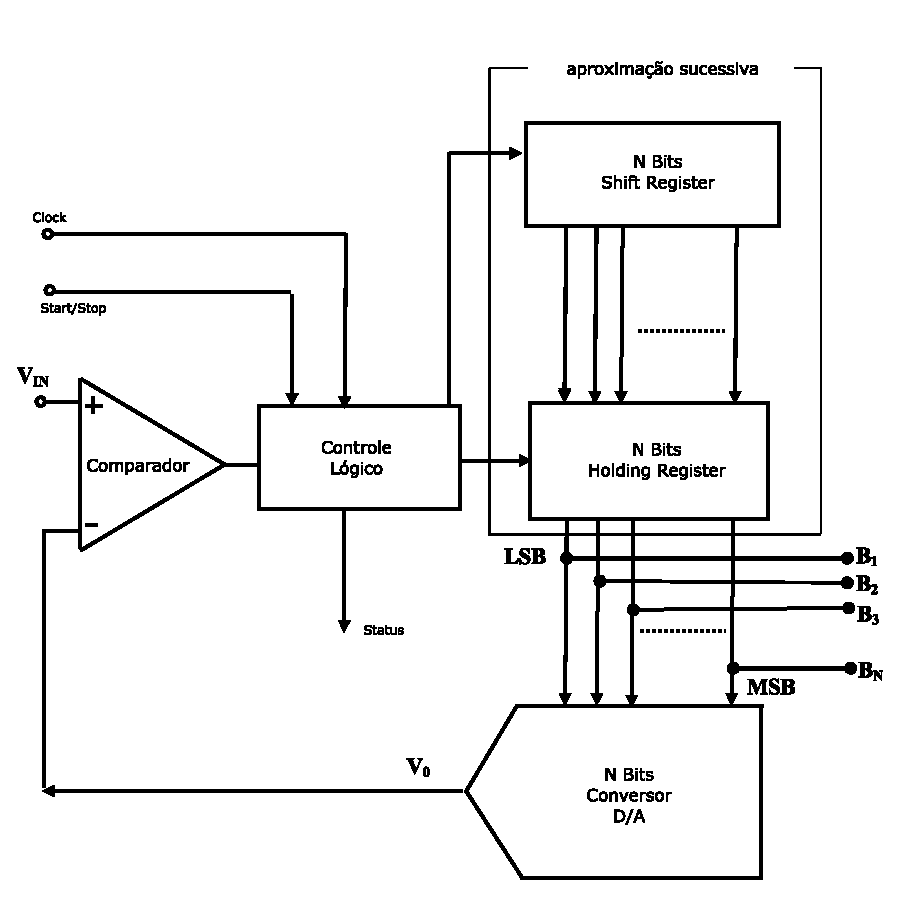
\includegraphics[width=0.9\textwidth] {figuras/ConversorAD.eps}}
	\caption{Conversor A/D tipo Aproximação Sucessiva}
	\label{fig:ConversorAD}
\end{figure}

Como podemos ver na figura \ref{fig:ConversorAD} este conversor utiliza a técnica de realimentação para relacionar uma voltagem analógica de entrada com um código digital, através de um conversor DA (\emph{Digital-To-Analog Converter}) e um comparador. O processo de conversão inicia quando o \emph{Shift Register} e o \emph{Holding Register} são zerados, e então o MSB do \emph{Holding Register} vai para nível alto. Então o comparador relaciona a saída do conversor DA com a tensão $V_{IN}$, se $V_{O} < V_{IN}$ a conversão chega ao fim, porém se isso não for verdade a etapa se repete porém MSB vai para nível baixo e o segundo SB vai para nível alto. E assim se dá a conversão. 


O Tiva TM4C1294NCPDT possui 2 módulos de conversão AD  de 12-bit, que podem ser usados em qualquer um das 20 entradas de sinal analógico. É possível realizar amostragens sequenciais entre os canais ou no mesmo canal repetidamente com intervalos de tempo  programáveis. Cada módulo AD possui 8 comparadores que possibilitam realizar comparações entre os sinais de entrada e  valores pré-definidos, para que assim possa ser realizado as mais diversas operações.  Ainda é possível usar um \emph{trigger} diferente para cada um dos módulos, ou usar um \emph{trigger} para acionar ambos os módulos.

A tabela \ref{tab:CanaisADC} apresenta os pinos de entrada para os módulos ADC0 e ADC1, com a descrição do nome do pino de entrada, o numero referente a este pino, sua função e o tipo de \emph{buffer} usado. Nesta mesma tabela temos o  pino chamado de $VREFA+$ que é o pino da tensão de referência usado pelo AD. A $VREFA+$ corresponde o valor máximo que o conversor DA, usado pelo AD para realizar a comparação com a tensão de entrada, pode atingir. 

A tensão $VREFA+$ é extremamente importante para se realizar a conversão AD, pois se este valor não for selecionado de forma adequada pode-se acarretar problemas no valor digital. $VREFA+$ ela pode ser alternada entre uma fonte de referência interna ou externa. 

\begin{center}
\begin{longtable}{|c|c|c|c|c|c|}
	\rowcolor[HTML]{000000}
	{\color[HTML]{FFFFFF} Pino} & {\color[HTML]{FFFFFF} $n^{o}$} & {\color[HTML]{FFFFFF} Mux/Função} & {\color[HTML]{FFFFFF} Tipo} & {\color[HTML]{FFFFFF} Buffer} & {\color[HTML]{FFFFFF} Descrição}            \\
	AIN0                        & 12                             & PE3                               & I                           & Analógico                     & ADC - Entrada 0                             \\
	\hline
	AIN1                        & 13                             & PE2                               & I                           & Analógico                     & ADC - Entrada 1                             \\
	\hline
	AIN2                        & 14                             & PE1                               & I                           & Analógico                     & ADC - Entrada 2                             \\
	\hline
	AIN3                        & 15                             & PE0                               & I                           & Analógico                     & ADC - Entrada 3                             \\
	\hline
	AIN4                        & 128                            & PD7                               & I                           & Analógico                     & ADC - Entrada 4                             \\
	\hline
	AIN5                        & 127                            & PD6                               & I                           & Analógico                     & ADC - Entrada 5                             \\
	\hline
	AIN6                        & 126                            & PD5                               & I                           & Analógico                     & ADC - Entrada 6                             \\
	\hline
	AIN7                        & 125                            & PD4                               & I                           & Analógico                     & ADC - Entrada 7                             \\
	\hline
	AIN8                        & 124                            & PE5                               & I                           & Analógico                     & ADC - Entrada 8                             \\
	\hline
	AIN9                        & 123                            & PE4                               & I                           & Analógico                     & ADC - Entrada 9                             \\
	\hline
	AIN10                       & 121                            & PB4                               & I                           & Analógico                     & ADC - Entrada 10                            \\
	\hline
	AIN11                       & 120                            & PB5                               & I                           & Analógico                     & ADC - Entrada 11                            \\
	\hline
	AIN12                       & 4                              & PD3                               & I                           & Analógico                     & ADC - Entrada 12                            \\
	\hline
	AIN13                       & 3                              & PD2                               & I                           & Analógico                     & ADC - Entrada 13                            \\
	\hline
	AIN14                       & 2                              & PD1                               & I                           & Analógico                     & ADC - Entrada 14                            \\
	\hline
	AIN15                       & 1                              & PD0                               & I                           & Analógico                     & ADC - Entrada 15                            \\
	\hline
	AIN16                       & 18                             & PK0                               & I                           & Analógico                     & ADC - Entrada 16                            \\
	\hline
	AIN17                       & 19                             & PK1                               & I                           & Analógico                     & ADC - Entrada 17                            \\
	\hline
	AIN18                       & 20                             & PK2                               & I                           & Analógico                     & ADC - Entrada 18                            \\
	\hline
	AIN19                       & 21                             & PK3                               & I                           & Analógico                     & ADC - Entrada 19                            \\
	\hline
	&                                &                                   &                             &                               & A tensão de referência                      \\
	&                                &                                   &                             &                               & \multicolumn{1}{l|}{é usada pelo AD para}    \\
	&                                &                                   &                             &                               & \multicolumn{1}{l|}{fixar o valor máximo de} \\
	\multirow{-4}{*}{VREFA+}    & \multirow{-4}{*}{9}            & \multirow{-4}{*}{fixo}            & \multirow{-4}{*}{-}         & \multirow{-4}{*}{Analógico}   & \multicolumn{1}{l|}{conversão.}  \\ 
	\hline
	\caption{Canais de Entrada ADC - Tiva TM4C1294NCPDT \cite{DATASHEET_TIVA} }
	\label{tab:CanaisADC}
\end{longtable}
\end{center}
